%%%%%%%%%%%%%%%%%%%%%%%%%%%%%%%%%%%%%%%%%%%%%%%%%%%%%%%%%%%%%%%%%%%%%%%%%%%%%%%%
\subsection{LabVIEW 2022}

LabVIEW (Laboratory Virtual Instrument Engineering Workbench) is a system-design platform and development environment for visual programming created and owned by National Instruments. Currently, the experiment uses the 2015 version of LabVIEW for the development of the VITO control system on the PXI. Starting in 2022, NI software moved to a subscription model \cite{ni}. This means that in order to update the current version of LabVIEW used in the experiment to the newest, subscription-based version (2022 and beyond), so that the software framework used in the experiment does not become outdated, a costly annual fee becomes inevitable.

From this arose the problem that my internship was centered around. That is, is it feasible to migrate the software development environment from LabVIEW, a proprietary visual programming language, to open-source languages, such as Python or C? And if so, what are the critical steps of such a migration process?

In the ideal situation where LabVIEW can be successfully replaced, not only will the cost of experimental operations be reduced by avoiding the annual subscription fee, the development process of necessary software programs also has the potential of becoming more efficient, making digital and analog I/O processes more adaptable to changing experimental needs.

Since LabVIEW is used to develop software programs for digital and analog I/O modules, it is then necessary to investigate whether and which open-source programming languages are viable alternatives for each module.

%%%%%%%%%%%%%%%%%%%%%%%%%%%%%%%%%%%%%%%%%%%%%%%%%%%%%%%%%%%%%%%%%%%%%%%%%%%%%%%%
\subsection{NI PXI-6713 Analog Output}

The NI PXI-6713 Analog Output module is a 12-bit, 8-channel, 1 MS/s high-speed ``simple" card designed to deliver simultaneous, multichannel updates for control and waveform output applications, such as stimulus-response, power supply control, high-speed, deterministic control, and sensor/signal simulation. It is considered a ``simple" module because it does not contain a field-programmable gate array (FPGAs are elaborated in Section \ref{sec:2_1_fpga_hdl}) that must be programmed by a hardware language to execute desired functions.

This module is controlled by the NI-DAQmx instrument driver, which allows the configuration and programming of the DAQ system from low-level OS and device control to high-level programming languages. Currently, for the experiment, programs for the NI PXI-6713 Analog Output module are developed in LabVIEW, which integrates the NI-DAQmx driver. Fortunately, NI-DAQmx can also be used with Python, C, and other languages, which is exactly what we need for software migration.

One of my internship objectives was to translate sample NI-DAQmx programs already written in LabVIEW to Python and C. The reason was to familiarize myself with LabVIEW, to examine the compatibility of such language migration, and to conduct runtime tests comparing the speeds of the translated programs between the two open-source languages. The two sample LabVIEW programs chosen were \textbf{OnDemand}, which configures the NI PXI-6713 module to output a continuous, constant signal voltage, and \textbf{Finite}, which configures the module to output a finite, periodical signal voltage.

\begin{table}[h!]
    \begin{minipage}[t]{.475\linewidth}
        \centering
        \begin{tabular}{ p{2.5cm} | p{2.25cm} | p{2.25cm} }
            \hline
            \multirow{2}{*}{\textbf{OnDemand}} & \multicolumn{2}{c}{Average Runtime (ms)} \\
            \cline{2-3}
            & $V_{out} = 5$ V & $V_{out} = 7.5$ V \\
            \hline
            Python & 2.085 & 2.130 \\
            \hline
            C & 1.904 & 1.800 \\
            \hline
        \end{tabular}
        \caption*{a. Average runtimes for the LabVIEW OnDemand program translated to Python and C. Each average runtime was calculated over 10 separate tests, with 10,000 runs per test. The constant, on-demand ouput analog voltage was set at 5 V and 7.5 V for different tests.}
        \label{tab:runtime_on_demand}
    \end{minipage}
    \hspace{.025\linewidth}
    \begin{minipage}[t]{.475\linewidth}
        \centering
        \begin{tabular}{ p{2cm} | p{2.5cm} | p{2.5cm} }
            \hline
            \multirow{2}{*}{\textbf{Finite}} & \multicolumn{2}{c}{Average Runtime (ms)} \\
            \cline{2-3}
            & $f = 0.1$ MHz & $f = 1$ MHz \\
            \hline
            Python & 21.450 & 21.538 \\
            \hline
            C & 20.020 & 20.976 \\
            \hline
        \end{tabular}
        \caption*{b. Average runtimes for the LabVIEW Finite program translated to Python and C. Each average runtime was calculated over 10 separate tests, with 1,000 runs per test. The sample time was fixed to 10 ms for all runs, while the sampling rate $f$ was set to 0.1 MHz and the recommended maximum of 1 MHz for different tests.}
        \label{tab:runtime_finite}
    \end{minipage}
    \caption{}
    \label{tab:runtime}
\end{table}

With the help of APIs (application programming interfaces) and tutorial programs provided by NI \cite{ni_nidaqmx_python}\cite{ni_nidaqmx_c} as references, I successfully translated these two simple NI-DAQmx programs from LabVIEW to Python and C and performed runtime tests. The runtime results are summarized in Table \ref{tab:runtime}.

The results show that the sample LabVIEW programs translated to C generally have a slightly faster runtime compared to those translated to Python. Although OnDemand and Finite are quite simple in complexity, we can generalize this result beyond these two sample programs. This is because the Python NI-DAQmx package was implemented as a complex, highly object-oriented wrapper around the NI-DAQmx C API using the \textbf{ctypes} Python library \cite{ni_nidaqmx_python}.

Consequently, when migrating LabVIEW programs that configure the NI PXI-6713 Analog Output module, both Python and C are viable open-source language alternatives. C provides a faster runtime as it is more primitive than Python, while Python is generally easier to learn, code, and debug.

%%%%%%%%%%%%%%%%%%%%%%%%%%%%%%%%%%%%%%%%%%%%%%%%%%%%%%%%%%%%%%%%%%%%%%%%%%%%%%%%
\subsection{NI 6581 Digital I/O \& NI 5761 Analog Input}

The NI 6581 Digital I/O \& NI 5761 Analog Input modules are ``smart" cards because they provide wider ranges of customizable functions via their respective on-board FPGA. Figure \ref{fig:ch1_schematics} shows the software and hardware schematics of how such an FPGA works in these two modules.

\begin{figure}[ht]
    \centering
    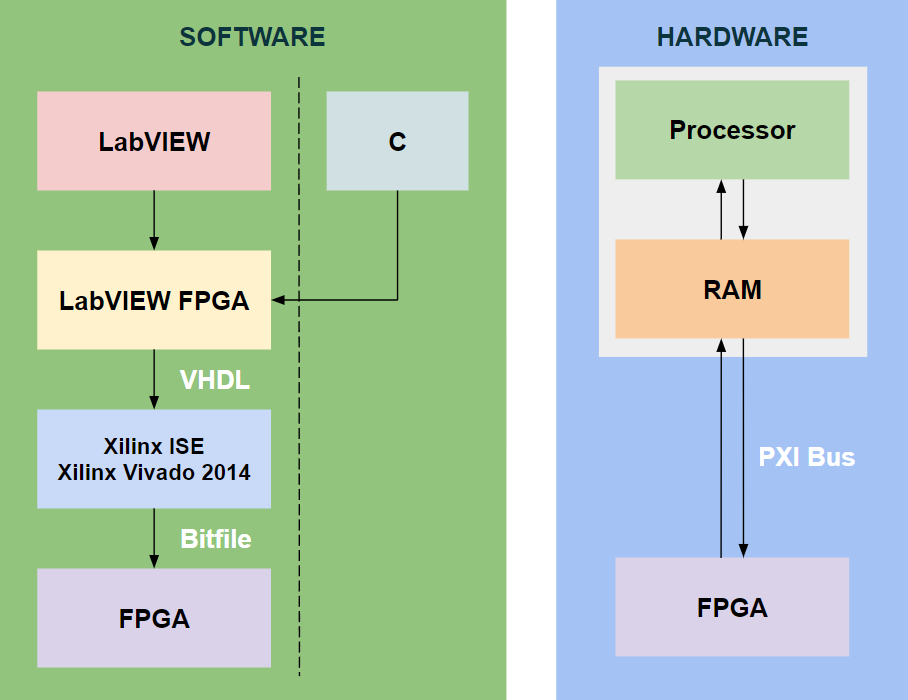
\includegraphics[width=0.75\columnwidth]{images/chapter_1/schematics.png}
    \caption{Schematics of software and hardware communication processes for NI ``smart" modules. On the software side, the FPGA is programmed by a bitfile generated using Xilinx Vivado environment application. The bitfile corresponds to a hardware design program written in a hardware description language (HDL), such as Verilog or VHDL. This hardware design is then communicated via the LabVIEW FPGA software module to LabVIEW or C programs for front-end purposes. On the hardware side, the FPGA communicates with the on-board RAM (random access memory) via the PXI bus, and a processor works with the data stored in the RAM.}
    \label{fig:ch1_schematics}
\end{figure}

For both the NI 6581 Digital I/O and the NI 5761 Analog Input modules, the files that describe how the FPGA communicates with the RAM via the PXI bus was encrypted by NI for proprietary reasons. This introduced a bottleneck in our endeavor as it prevented us from replacing LabVIEW with Python or C like it could easily be done for the NI PXI-6713 Analog Output module. As a result, we must look into alternative FPGA-based devices for digital I/O and analog input that could replace these two ``smart" modules and hopefully relieve the experiment from such a proprietary stranglehold.